\section{Introduction}
\begin{enumerate}
	\item UAV's
	\item Smart Cities
	\item What more?
\end{enumerate}

\section{Related Literature}
\begin{enumerate}
	\item ant algorithms for UAV / Path planning
	\item path planning with multiple depots / battery
	\item ...
\end{enumerate}

\section{Optimization Problem}
\begin{enumerate}
	\item multiple depots
	\item drones have to recharge and thus deviate from their actual route
	\item ...
	
\end{enumerate}

\section{Algorithm}
This section describes the optimization algorithm used for path-finding in the previously described problem domain.

\subsection{Background}
The algorithm that is used to optimize the path-finding and item delivery is inspired by the Ant Colony Algorithm. This algorithm was originally proposed by Marco Dorigo in 1992 \cite{dorigo.1992}. The Ant Colony Algorithm describes how ants find the shortest path between the colony and a source of food (see Figure \ref{fig:algo_dreo.2016}). The search for the shortest path is conducted in multiple steps. In the first step an ant finds a food source (F) and during its way back to the colony (N) the ant lays a pheromone trail. In the next step, other ants might find the same food source and also lay down a trail of pheromones. Other ants might follow different pheromone trails to the food source and drop pheromones as well. Since the ants that walk the shortest path can traverse the route more often than ants that follow a longer path, the pheromone level on the shorter path is higher than the level on other paths. As a result, more and more ants favour the shorter path (3rd step).

\begin{figure}[htbp]\label{fig:algo_dreo.2016}
	\centering
	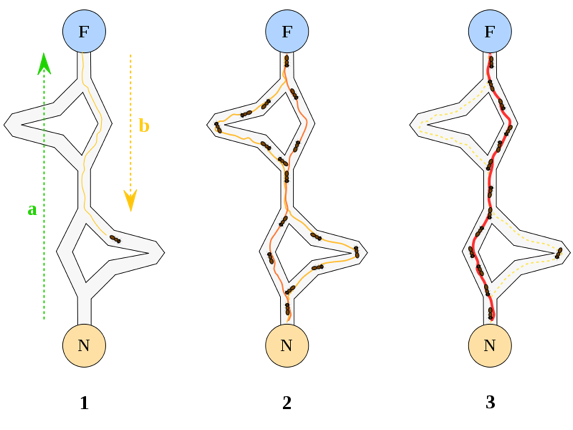
\includegraphics[width=0.6\textwidth]{images/algorithm_Picture1.png}
	\caption{Shortest path find by an ant colony Source: \url{https://de.wikipedia.org/wiki/Datei:Aco_branches.svg}} 

\end{figure}


\subsection{Adaption}
In our use case we invert the Ant Colony Algorithm. Instead of using pheromones that attract, we employed repellents which are used to divert. Every time a UAV finds a non-optimal cell, it creates a repellent to let other UAVs know that it is not wise to include this cell on the route to find the target location. In the real world the pheromones decay over time. Each repellent has a strength which decreases over time.
The decay of repellents' strength is employed to avoid UAVs getting stuck in local optima because they cannot deliver an item to a location that is surrounded by repellents or the UAV itself is encompassed by repellents.

\subsection{Implementation}
In the first step the algoritm calculates all available steps. Available steps are defined as all neighboring cells that a UAV can visit from its current location (see Figure \ref{fig:algo_steps})
.
\begin{figure}[htbp]\label{fig:algo_steps}
	\centering
	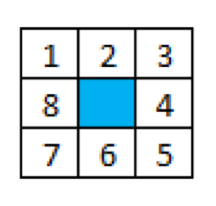
\includegraphics[width=0.3\textwidth]{images/algorithm_Picture2.png}
	\caption{All available steps a UAV can make (blue = UAV)} 
\end{figure}

To decide which of these available steps is the best, the euclidean distance to the target destination is calculated for each of the available steps. From these available steps, the cells that contain an obstacle are removed, as long as this obstacle is not a depot. Furthermore, the algorithm factors in repellents that might be in one or more of the available neighbouring cells.  
The calculated Euclidean distance is weighted with the current strength of a repellent:
\centering{
$
distance = distance + \frac{available_step.distance * repellent.strength}{100}
$}\newline
The weighted distance makes it more unlikely that the UAV will visit this cell. 
The cells are then added to the possible steps with their weighted distance.
After this second step, the possible steps are either cells that don't contain an obstacle other than a base station, empty cells and cells that contain a repellent. The possible steps are then sorted by distance.
\\
In the third step of the algorithm, the best step of the possible steps is selected. The best step is the step that has the lowest distance to the target cell. In the last step, the algorithm checks the last two steps the UAV has taken in order to identify sub-optimal routes (see Figure \ref{fig:algo_find_routes}).

\begin{figure}[htbp]\label{fig:algo_find_routes}
	\centering
	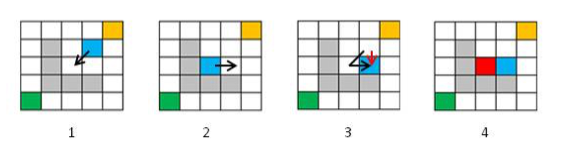
\includegraphics[width=0.6\textwidth]{images/algorithm_Picture3.png}
	\caption{Find sub-optimal routes and place repellents} 
\end{figure}

The UAV (blue) started at the base station (orange) and is on its way to deliver an item to a target location (green). When applying the algorithm, the UAV selects the cell that doptmizes the distance to the target location. As a result, the UAV moves to the bottom left neighbouring cell. In the second picture the UAV cannot move to the bottom left cell, because there is an obstacle. The next best cells are either to the left or the bottom. But again both cells are blocked by an obstacle. From the remaining three cells that are not blocked by an obstacle, the first two (right and top) have the same distance to the target destination and the third one has a higher distance to the target destination. Because of that, the UAV moves to the right. To find possible sub-optimal routes the last two steps of the UAV are checked (black arrow).
\\ 
The algorithm identifies that in order to reach the cell the UAV reached in picture 3, it could have taken a different path (red arrow). As a result, the UAV will place a repellent at the last cell (red square, picture4). If, for some reason, a UAV has visited a cell that contained a repellent and in the next step it becomes clear that the UAV took a sub-optimal path, it does not create a new repellent but instead resets the repellent's strength back to its initial value.

\section{Evaluation}
\begin{enumerate}
	\item Use KPI's that we defined
	\item Use graphics with cool Excel tables to present data
\end{enumerate}

\section{Conclusion}
\begin{enumerate}
	\item Overall summary
	\item limitations of this approach
	\item future development?
\end{enumerate}

\cite{Winery}